\documentclass{article}
\usepackage{amsmath}
\usepackage{amssymb}
\usepackage{graphicx}
\usepackage{hyperref}
\usepackage[version=4]{mhchem}


\begin{document}
\section*{Problem}
\(P A\) and \(P B\) are tangent to circle \(O\) at \(A\) and \(B\), respectively. \(A C\) is the diameter of circle \(O\). Prove: \(B C / / P O\).\\
\centering
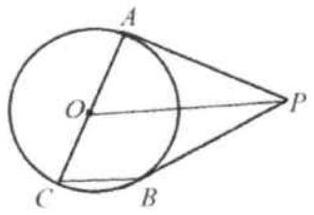
\includegraphics[width=\textwidth]{images/154(2).jpg}

\section*{Solution}
Method 1:\\
Connect \(O B\).\\
Since \(P A\) and \(P B\) are tangent to circle \(O, \triangle P A O \cong \triangle P B O\) \((O A=O B, P A=P B, P O=P O)\).\\
So \(\angle P O A=\angle B O B=\alpha\).\\
\(\angle P A O=90^{\circ}, \angle P D A=90^{\circ}\),\\
\(\angle A O B=2 \angle A C B\) (the measure of the central angle is twice\\
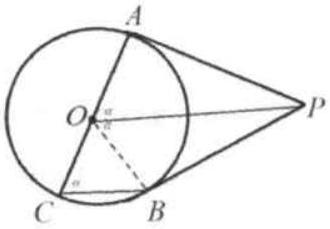
\includegraphics[width=\textwidth]{images/157.jpg} of the inscribed angle facing the same arc).\\
\(\angle C=\angle P O A=\alpha\).\\
Thus \(B C / / P O\).

\end{document}
